\subsection{Modelo U-Net}

En la figura \ref{fig:unet} se ilustra la arquitectura de una red del tipo U-Net. Este modelo consiste de dos partes, un encoder (lado izquierdo) y un decoder (lado derecho).  El encoder tiene una arquitectura típica de una red convolucional en la que cada paso se aplica una convolución de $3x3$ seguida de una capa con la función rectificador (ReLU) y otra capa con un max pooling de 2 dimensiones para una reducción de dimensión. En la etapa del decoder se aplica un aumento de dimensión seguida de una capa de convolución de 2x2. Al final se  concadena el resultado de este proceso con el mapa reducido. En seguida se aplica una serie de dos capas convolucionales de $3x3$ y se aplica la función ReLU. Al final del proceso se aplica una capa de convolución de $1x1$ que es usada para mapear cada componente a un número de canales. En total, la red tiene 23 capas convolucionales.

\begin{figure}[H]
    \centering
    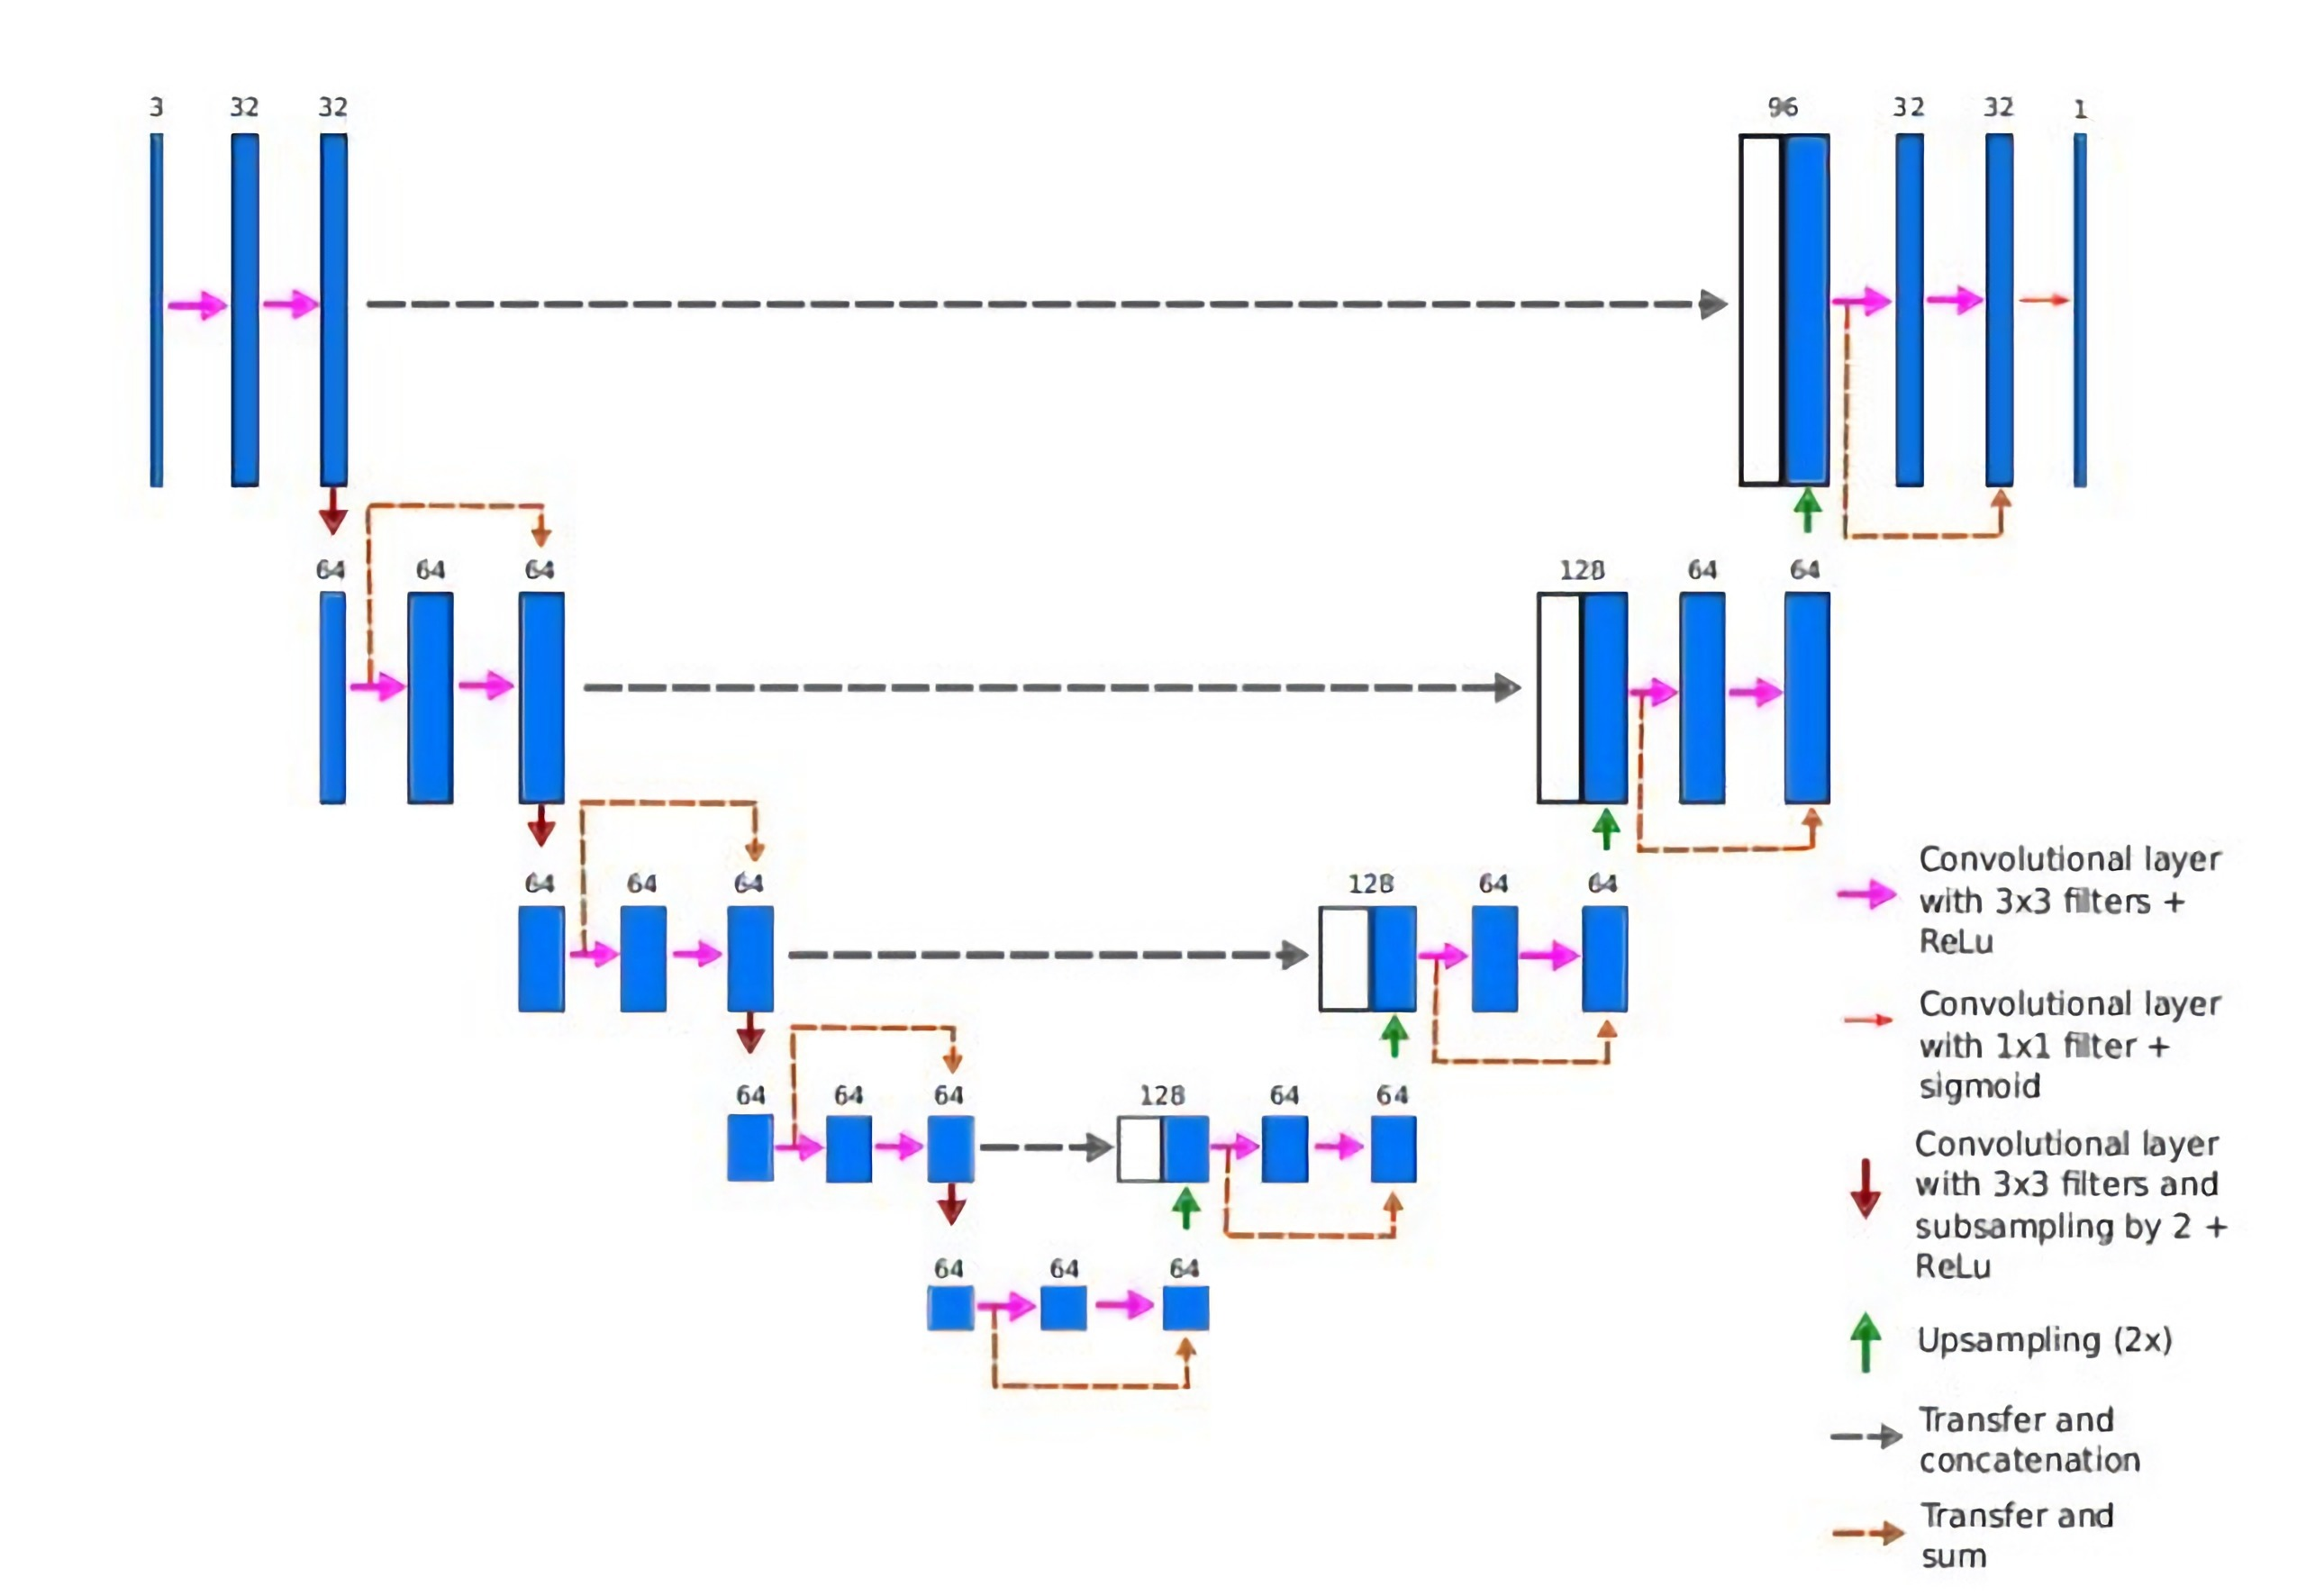
\includegraphics[width=13cm]{Graphics/unet_model.jpg}
    \caption{Arquitectura de una red del tipo U-Net.}
    \label{fig:unet}
\end{figure}